\chapter*{Задание №1}
Задание: процессы-сироты. В программе создаются не менее двух потомков. В потомках вызывается sleep(). Чтобы предок гарантированно завершился раньше своих потомков. Продемонстрировать с помощью соответствующего вывода информацию об идентификаторах процессов и их группе. Продемонстрировать «усыновление». Для этого надо в потомках вывести идентификаторы: собственный, предка, группы до блокировки и после блокировки.

\begin{lstlisting}[label = ordinary_min, caption=Процессы-сироты.]
#include <unistd.h>
#include <stdio.h>

#define FORK_ERROR -1
#define FORK_OK 0

#define COUNT_CHILDS 3

int main(void)
{
	pid_t childs_pid[COUNT_CHILDS];
	
	printf("Parent - pid: %d, pgrp: %d\n", getpid(), getpgrp());
	
	for (int i = 0; i < COUNT_CHILDS; i++)
	{
		pid_t child_pid = fork();
		if (child_pid == FORK_ERROR)
		{
			perror("Can't fork.\n");
			return 1;
		}
		else if (child_pid == FORK_OK)
		{
			printf("Child_%d born - pid: %d, ppid: %d, pgrp: %d\n", 
			       i + 1, getpid(), getppid(), getpgrp());
			sleep(2);
			printf("Child_%d is dead - pid: %d, ppid: %d, pgrp: %d\n",
			       i + 1, getpid(), getppid(), getpgrp());
			return 0;
		}
		else{
			childs_pid[i] = child_pid;
		}
		
	}
	
	printf("Parent-child_1_pid: %d, child_2_pid: %d, child_3_pid: %d\n", 
	        childs_pid[0], childs_pid[1], childs_pid[2]);
	printf("Parent process is dead.\n");
	
	return 0;
}
\end{lstlisting}


Результат работы программы представлен на рисунке \ref{png:res_1}:

\begin{figure}[H]
	\centering{
		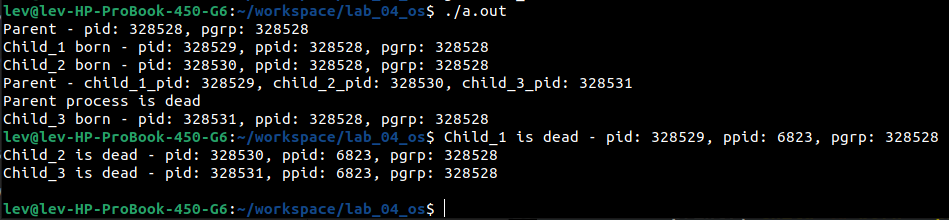
\includegraphics[scale=0.5]{../../../../../../../msys64/home/Лев/bmstu_sem_5_os/lab_04/report/images/task_1}
		\caption{Демонстрация работы программы (задание 1).}
		\label{png:res_1}}
\end{figure}